\documentclass[conference]{IEEEtran}
\usepackage{graphicx}
\usepackage{booktabs}
\usepackage{siunitx}
\usepackage{url}
\usepackage[hidelinks]{hyperref}
\graphicspath{{figs/}}
\newcommand{\SvrMed}{9.2}
\newcommand{\SvrNinety}{35.7}
\newcommand{\UnwMed}{16.7}
\newcommand{\UnwNinety}{58.7}
\newcommand{\UnwOver}{2.7}
\newcommand{\SvrOver}{0.06}
\newcommand{\SvrBetterAll}{every}
\newcommand{\LocMed}{11.0}
\newcommand{\LocMean}{13.4}
\newcommand{\LocNinety}{22.0}
\newcommand{\LocMax}{54.4}
\newcommand{\LocBest}{3.8}
\newcommand{\LocBestExp}{6}
\newcommand{\LocWorst}{20.4}
\newcommand{\LocWorstExp}{1}

\makeatletter\newcommand{\rawinput}[1]{\@@input #1 }\makeatother
\sisetup{detect-all}

\begin{document}

\title{Multi-Tag Ranging and Localization: Evaluation}
\author{\IEEEauthorblockN{Manavjeet Singh}}
\maketitle

\section{Evaluation Setup}

\subsection{Deployments}
We evaluate on 12 indoor deployments (Exp.~1--12). Each deployment places
12 or 15 tags on vertical poles in an area with sides of
\SI{0.99}{m} to \SI{1.75}{m} (Table~\ref{tab:setup}).
Fig.~\ref{fig:photos} shows Exp.~10. Fig.~\ref{fig:layouts} shows the layout of every
deployment.

\begin{figure}[t]
  \centering
  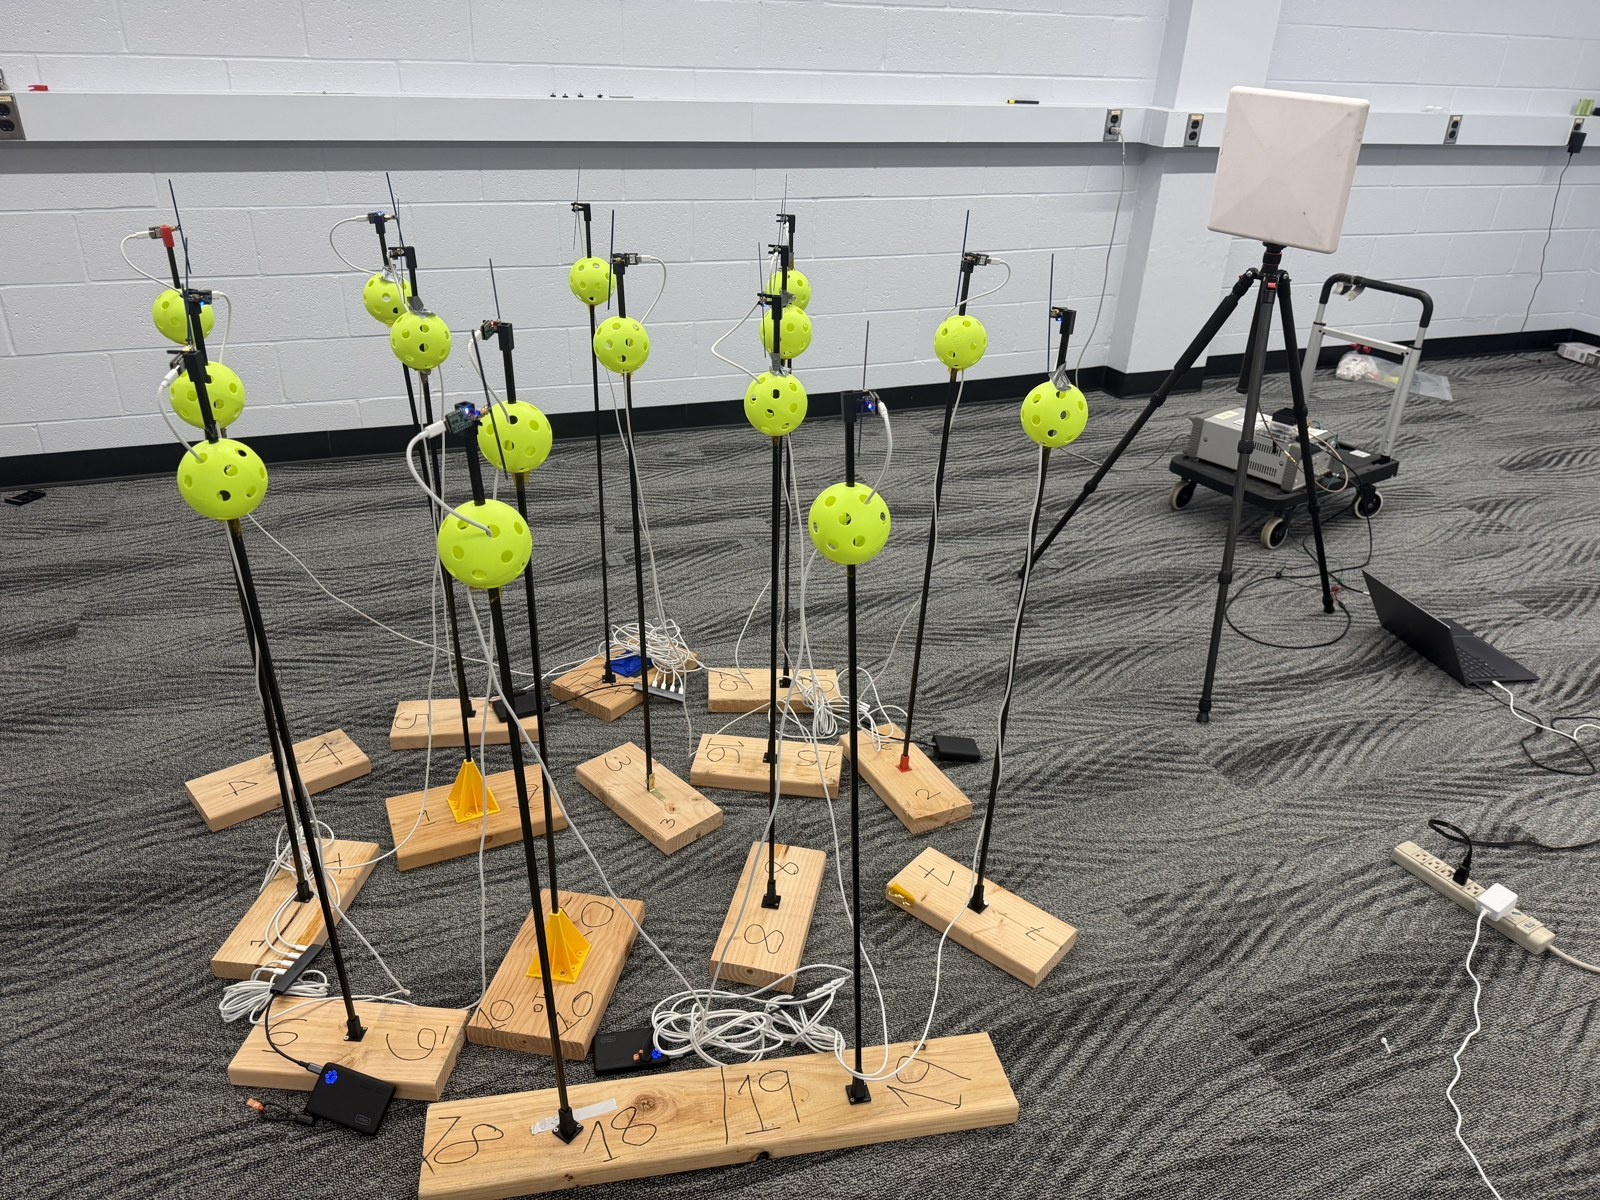
\includegraphics[width=0.49\columnwidth]{photo_a.jpg}\hfill
  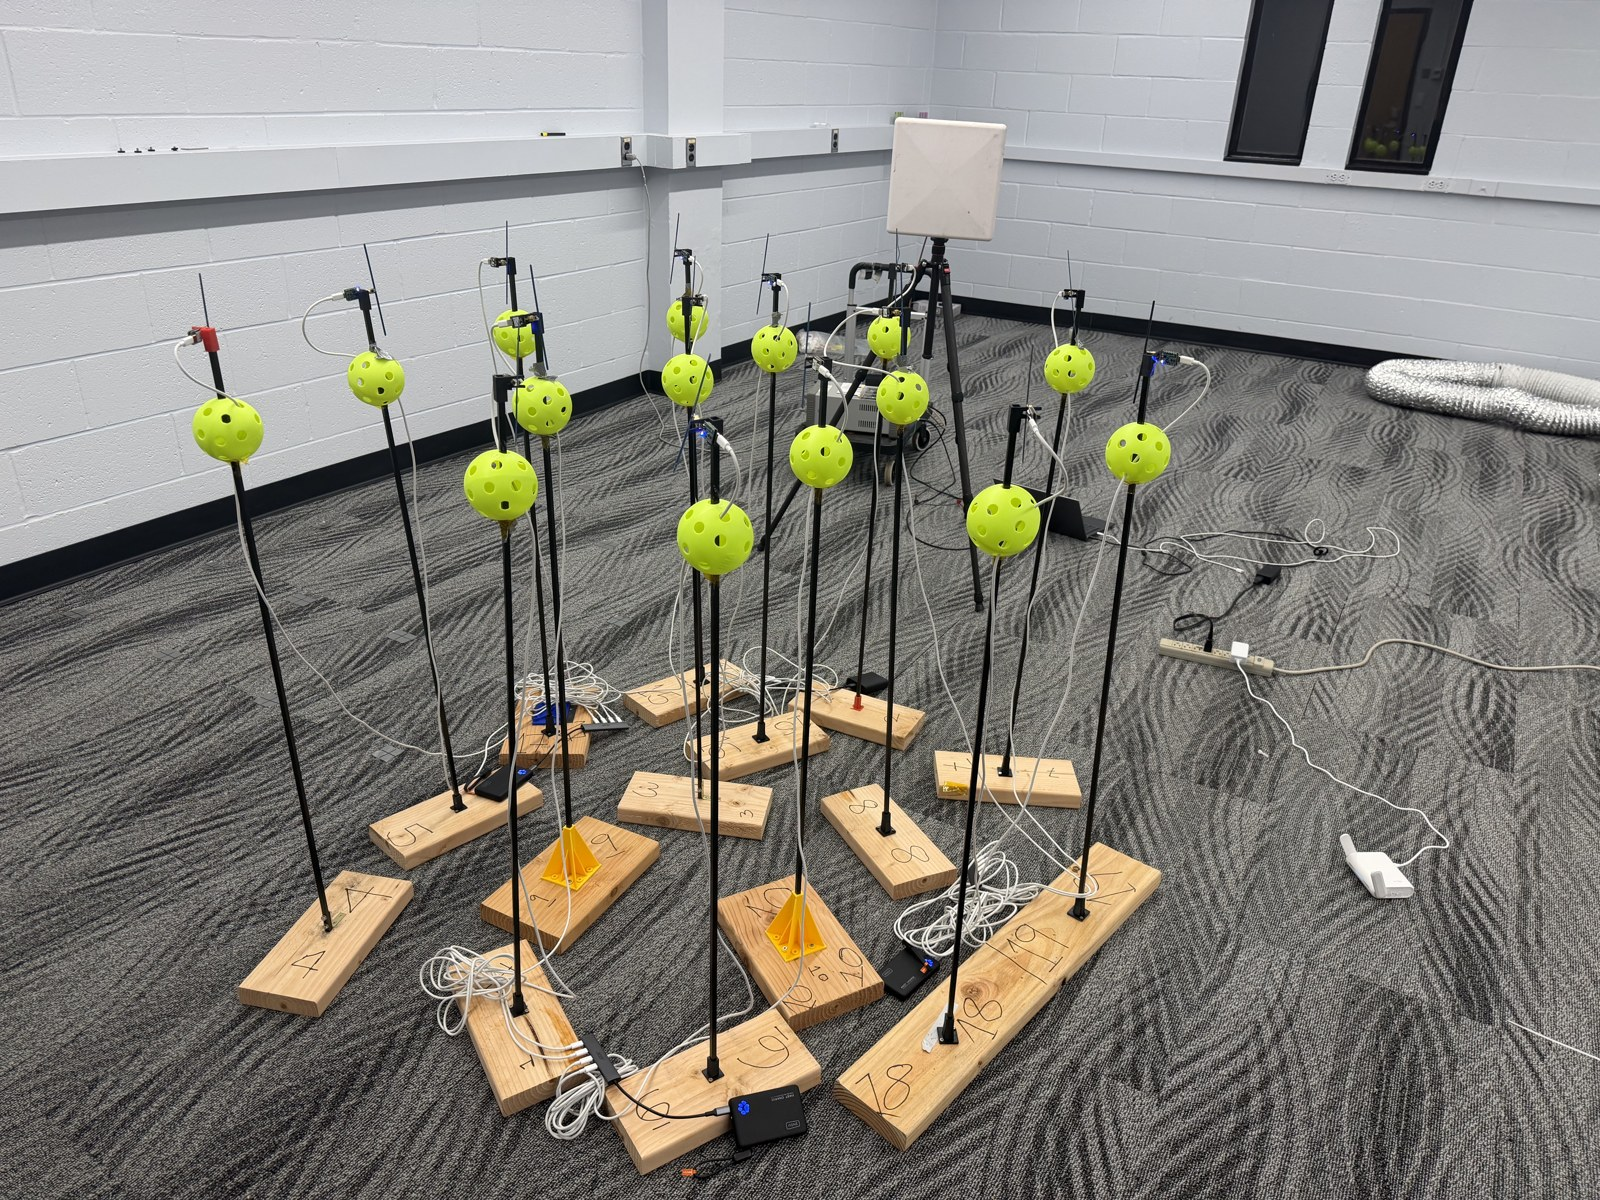
\includegraphics[width=0.49\columnwidth]{photo_b.jpg}
  \caption{Deployment of Exp.~10 (15 tags), viewed from two sides.}
  \label{fig:photos}
\end{figure}

\subsection{Ground truth}
Tag positions are taken from a 3D scan of each deployment. Ground-truth link
distances are the 3D distances between tags. Localization is evaluated in the horizontal ($x$, $y$) plane.

\subsection{Measurements}
Every tag pair (link) is measured at 18 carrier frequencies from \SI{775}{MHz}
to \SI{955}{MHz} in \SI{10}{MHz} steps (\SI{815}{MHz} excluded), giving a
\SI{180}{MHz} span. Each link is measured in 3 runs. All links are measured:
66 per deployment with 12 tags and 105 per deployment with 15 tags, 909 links
and 2727 link measurements in total.

Link distances range from \SI{0.21}{m} to \SI{1.90}{m}, with a median of
\SI{0.73}{m} (Fig.~\ref{fig:linkdist}).

\begin{figure}[t]
  \centering
  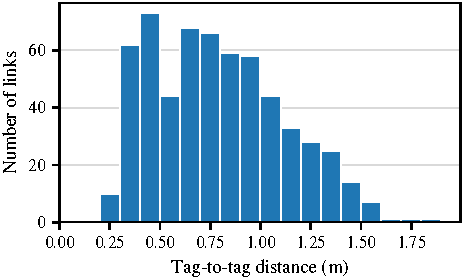
\includegraphics[width=\columnwidth]{link_dist.pdf}
  \caption{Distribution of ground-truth tag-to-tag distances over all 909 links
  of Exp.~1--12 (bin width \SI{0.1}{m}).}
  \label{fig:linkdist}
\end{figure}

\begin{figure}[t]
  \centering
  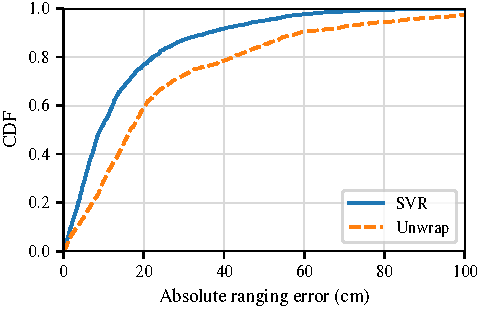
\includegraphics[width=\columnwidth]{ranging_cdf.pdf}
  \caption{CDF of absolute tag-to-tag ranging error, SVR vs.\ Unwrap, over 2727
  link measurements (909 links $\times$ 3 runs) from Exp.~1--12. The $x$-axis is
  cut at \SI{100}{cm}; \UnwOver\% of Unwrap errors and \SvrOver\% of SVR errors exceed it.}
  \label{fig:ranging}
\end{figure}

\begin{figure*}[t]
  \centering
  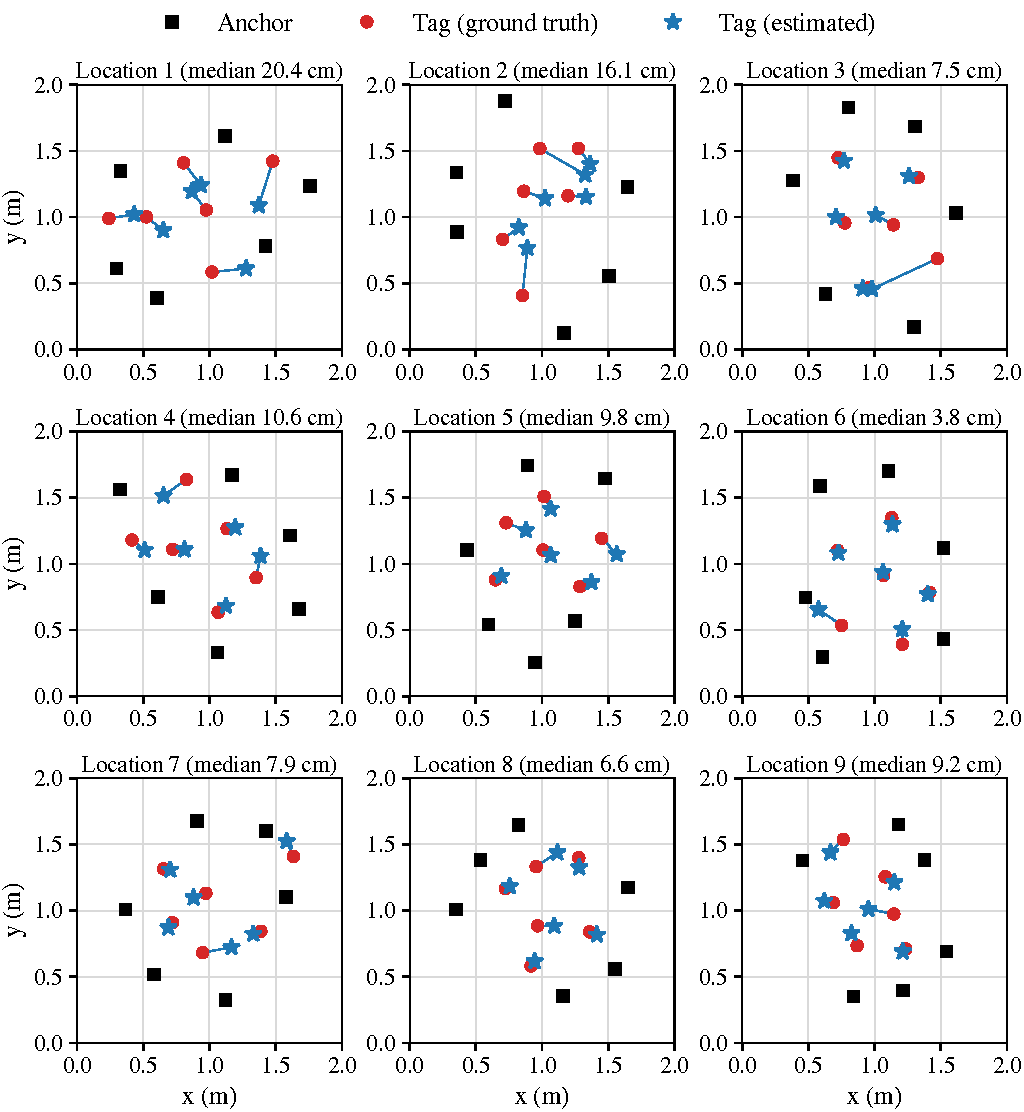
\includegraphics[width=\textwidth]{layouts.pdf}
  \caption{Layouts of Exp.~1--12 in the horizontal plane. Squares: anchors.
  Circles: true positions of localized tags. Stars: positions estimated by the
  merged method; each line joins a tag's true and estimated positions. All panels
  use the same scale.}
  \label{fig:layouts}
\end{figure*}

\begin{figure}[!t]
  \centering
  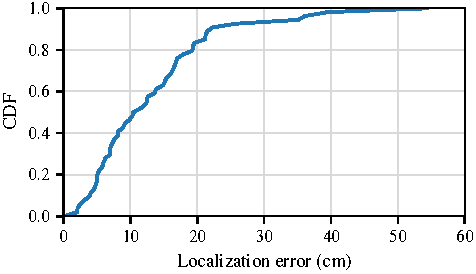
\includegraphics[width=\columnwidth]{loc_cdf.pdf}
  \caption{CDF of 2D localization error of the merged method over the 81
  localized tags of Exp.~1--12 (6 anchors per deployment).}
  \label{fig:loc}
\end{figure}

\subsection{Ranging protocol}
Ranging follows~\cite{ranging}. SVR is evaluated with leave-one-experiment-out
cross-validation: the model for each experiment is trained on the other
experiments only. A 13th deployment, not reported here, is used only as training
data. Unwrap requires no training. Each of the 2727 link measurements is one test
sample.

\subsection{Localization protocol}
Localization follows~\cite{loc} and uses the SVR ranges as input. In each
deployment, 6 tags are anchors with known positions; the remaining 6 or 9 tags
are localized (81 tags in total). The anchors are the 6 tags whose convex hull
has the largest area, so the anchors lie on the perimeter of the deployment.

\section{Results}

\subsection{Ranging accuracy}
Fig.~\ref{fig:ranging} compares the absolute ranging error of SVR and Unwrap over
all 2727 link measurements. SVR has a median error of \SI{\SvrMed}{cm} and a
90th-percentile error of \SI{\SvrNinety}{cm}. Unwrap has a median error of
\SI{\UnwMed}{cm} and a 90th-percentile error of \SI{\UnwNinety}{cm}. SVR has the lower
median error in \SvrBetterAll{} deployment (Table~\ref{tab:setup}).

\subsection{Localization accuracy}
Fig.~\ref{fig:loc} shows the localization error of the 81 localized tags. The
median error is \SI{\LocMed}{cm}, the mean is \SI{\LocMean}{cm}, the 90th percentile
is \SI{\LocNinety}{cm}, and the maximum is \SI{\LocMax}{cm}. Per-deployment medians (Table~\ref{tab:setup}) range
from \SI{\LocBest}{cm} (Exp.~\LocBestExp) to \SI{\LocWorst}{cm} (Exp.~\LocWorstExp).
Fig.~\ref{fig:layouts} shows the estimated position of every tag.

\begin{table*}[t]
  \centering
  \caption{Deployments and per-deployment median errors. Distances are
  ground-truth tag-to-tag distances.}
  \label{tab:setup}
  \begin{tabular}{@{}r rrrr rrr rr rr r@{}}
    \toprule
    & \multicolumn{4}{c}{Nodes} & \multicolumn{3}{c}{Link distance (\si{m})} &
      \multicolumn{2}{c}{Extent (\si{m})} &
      \multicolumn{2}{c}{Ranging error (\si{cm})} & Loc.\ error \\
    \cmidrule(lr){2-5}\cmidrule(lr){6-8}\cmidrule(lr){9-10}\cmidrule(lr){11-12}
    Exp. & Tags & Anchors & Localized & Links & Min & Median & Max & $x$ & $y$ &
      SVR & Unwrap & (\si{cm}) \\
    \midrule
    \rawinput{table_rows.tex}
    \bottomrule
  \end{tabular}
\end{table*}

\begin{thebibliography}{1}
\bibitem{ranging}
M.~Singh, Y.~Xie, A.~Ahmad, M.~Stana\'cevi\'c, S.~R.~Das, and P.~M.~Djuri\'c,
``Tag-to-tag range estimation for passive backscattering tags,'' in
\emph{Proc. 18th Int. Conf. Communication Systems and Networks (COMSNETS)},
Bengaluru, India, Jan. 2026, pp.~980--984,
doi: \href{https://doi.org/10.1109/COMSNETS67989.2026.11418103}{10.1109/COMSNETS67989.2026.11418103}.
\bibitem{loc}
M.~Singh, Y.~Xie, A.~Ahmad, M.~Stana\'cevi\'c, S.~R.~Das, and P.~M.~Djuri\'c,
``Sub-decimeter range estimation and localization for passive backscattering
tag-to-tag networks,'' unpublished manuscript, under revision for
\emph{ACM Trans. Internet of Things}, 2026.
\end{thebibliography}

\end{document}
